\subsection{Hubble Constant from \texorpdfstring{$\chi$}{χ} Dynamics}
  \label{subsec:hubble-constant-from-chi-dynamics}

  An implication of the relaxation dynamics developed in
  Section~\ref{subsec:emergent-hubble-law} is that, in Cosmochrony,
  the Hubble parameter is not introduced as a free cosmological constant, but arises
  as an effective quantity associated with the irreversible relaxation of the
  $\chi$ substrate.

  At the level of an effective spacetime description, it may be written as
  \begin{equation}
    H(t) = \frac{\dot{\chi}}{\chi},
  \end{equation}
  where the dot denotes differentiation with respect to an effective cosmological
  time parameter introduced solely to parametrize the relaxation ordering, not a
  fundamental temporal evolution.

  In homogeneous regimes, the relaxation rate approaches its maximal admissible
  value.
  Assuming $\dot{\chi}_{\mathrm{eff}} \simeq c$, the present-day Hubble parameter can
  be estimated as
  \begin{equation}
    H_0 \simeq \frac{c}{\chi(t_0)}.
  \end{equation}

  This relation establishes a direct correspondence between the observed Hubble
  constant and the characteristic relaxation scale of $\chi$ at the current epoch.
  Early-universe probes (such as CMB-based inferences) and late-time distance-ladder
  measurements effectively sample $\chi$ at different stages of its relaxation,
  naturally leading to systematically different inferred values of $H_0$ without
  invoking additional cosmological components or fine-tuned initial conditions.

  \paragraph{Resolution of the Hubble tension.}
    The modulation of the $\chi$ relaxation rate by large-scale matter
    inhomogeneities provides a natural mechanism for reconciling early-universe and
    late-time measurements of the Hubble constant.
    Within this framework, the effective Hubble parameter $H(z)$ acquires a mild
    redshift dependence that departs from the $\Lambda$CDM expectation at intermediate
    redshifts ($0.1 \lesssim z \lesssim 10$).
    This deviation reflects the partial projectability of the relaxation dynamics in
    inhomogeneous regimes, rather than the presence of additional cosmological
    components.
    The resulting behavior is directly testable through upcoming baryon acoustic
    oscillation and supernova surveys.

% Requires: \usepackage{pgfplots}
% Optional: \pgfplotsset{compat=1.18}
    \begin{figure}[t]
      \centering
      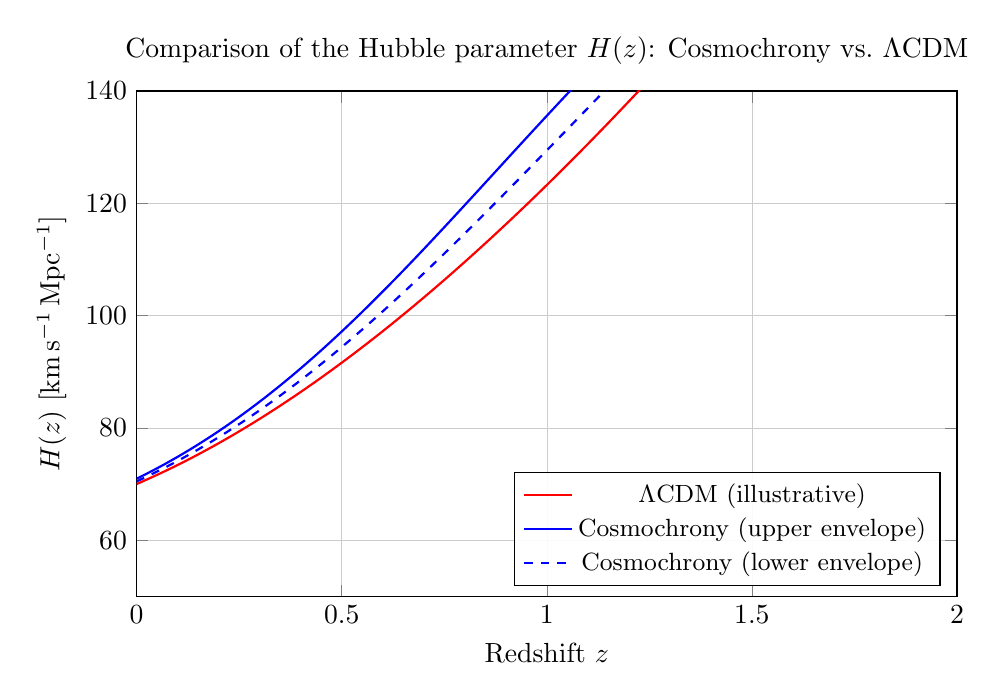
\begin{tikzpicture}
        \begin{axis}[
          width=12cm,
          height=8cm,
          title={Comparison of the Hubble parameter $H(z)$: Cosmochrony vs.\ $\Lambda$CDM},
        xlabel={Redshift $z$},
        ylabel={$H(z)$ [km\,s$^{-1}$\,Mpc$^{-1}$]},
        xmin=0, xmax=2,
        ymin=50, ymax=140,
        xtick={0,0.5,1,1.5,2},
        legend style={
          at={(rel axis cs:0.98,0.02)},
          anchor=south east,
          draw=black,
          fill=white,
          fill opacity=0.9,
          text opacity=1,
          font=\small
        },
        grid=both,
        grid style={line width=.1pt, draw=gray!10},
        major grid style={line width=.2pt, draw=gray!40},
        ]

          % --- Baseline LCDM ---
          \addplot[
            domain=0:2, samples=200,
            red, thick, mark=none
          ]
          {70*sqrt(0.3*(1+x)^3 + 0.7)};
          \addlegendentry{$\Lambda$CDM (illustrative)}

          % --- Cosmochrony band ---
          \addplot[
            domain=0:2, samples=200,
            blue, thick, mark=none
          ]
          {70*sqrt(0.3*(1+x)^3 + 0.7) * (1 + 0.10*exp(-2*(x-1)^2))};
          \addlegendentry{Cosmochrony (upper envelope)}

          \addplot[
            domain=0:2, samples=200,
            blue, thick, dashed, mark=none
          ]
          {70*sqrt(0.3*(1+x)^3 + 0.7) * (1 + 0.05*exp(-2*(x-1)^2))};
          \addlegendentry{Cosmochrony (lower envelope)}
        \end{axis}
      \end{tikzpicture}
      \caption{Schematic comparison of $H(z)$ in Cosmochrony and $\Lambda$CDM.
      Cosmochrony predicts a mild enhancement at intermediate redshifts due to
      relaxation inhomogeneities, providing a discriminating observational test.}
      \label{fig:hubble-comparison}
    \end{figure}
